% Results
%
%	some important things to know
% 	experimental parts in the chapter results
%	numerical results or so-called data
%	order of presentation
% 	cross references

\chapter{Results}

\section{Implemented System}

The implemented system consist of three pieces of software~:
\begin{enumerate}
	\item The software controlling the acquisition card in the machine.
	\item An acquisition software that run on a standard front-end Linux machine that is taking data during the \glspl{MD}.
	\item And an analyzing software that can compute the \glspl{FFT} on \glspl{GPU}.
\end{enumerate}

\begin{figure}[H]
\caption{Implemented acquisition software in the CERN infrastructure}
\centering
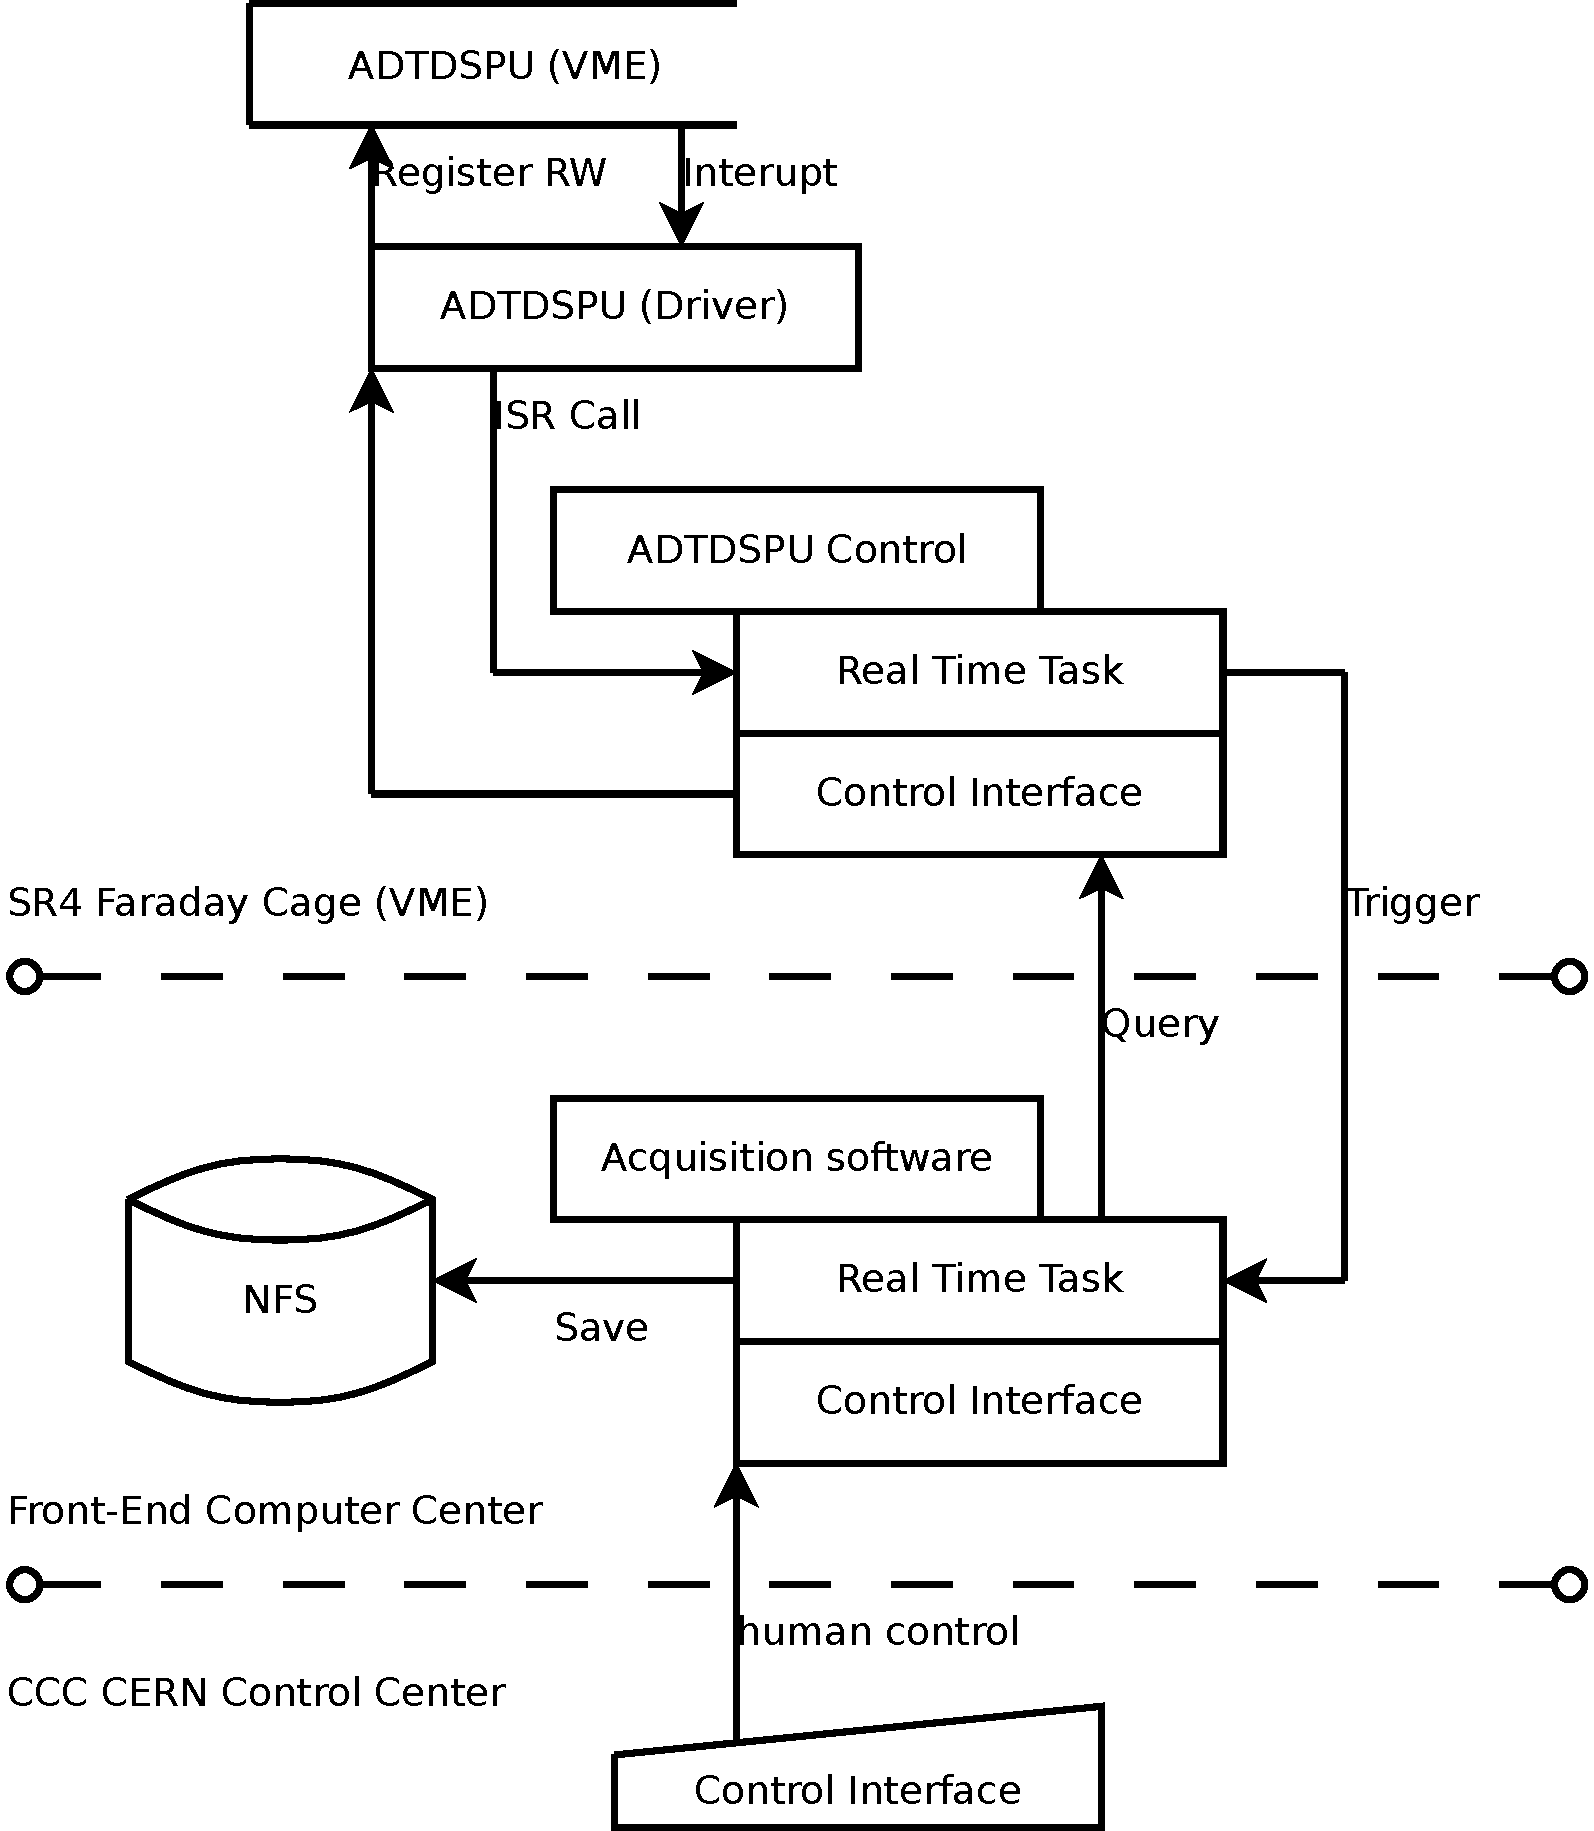
\includegraphics[scale=0.3]{ImplementedSoftFesa.pdf}
\end{figure}

In the final version the software will be merged in single executable that should run on the machine with the \gls{GPU} and the receiver card. The present solution has been put into place because the present hardware is still in development and there is no way of acquiring the maximum of 2880 bunches of the machine. The hardware is receiving the acquisition data but the \gls{VME} is not fast enough to transfer it to the \gls{CPU}.

	\subsection{ADTDSPU control software}

	The first layer that was needed is a driver that can control the \gls{VME} card and forward the interrupts. This is using the standard driver framework from the \gls{CO} at \gls{CERN}.

	The standard \gls{FESA}, the standard middle-ware framework used at \gls{CERN} to control equipment, was used to develop a higher level software to control the card. This particular card needs a real time task in order to react to an interrupt coming from the hardware and to inform when a new acquisition is ready to be read.

	\subsection{Acquisition software}

	The acquisition software was used to check that the idea of getting the tune out of the DSPU card data was feasible as well as providing a means to log the acquisition to a file for subsequent checking and processing.

	\begin{figure}[H]
	\caption{Tune acquisition software interface in FESA framework}
	\centering
	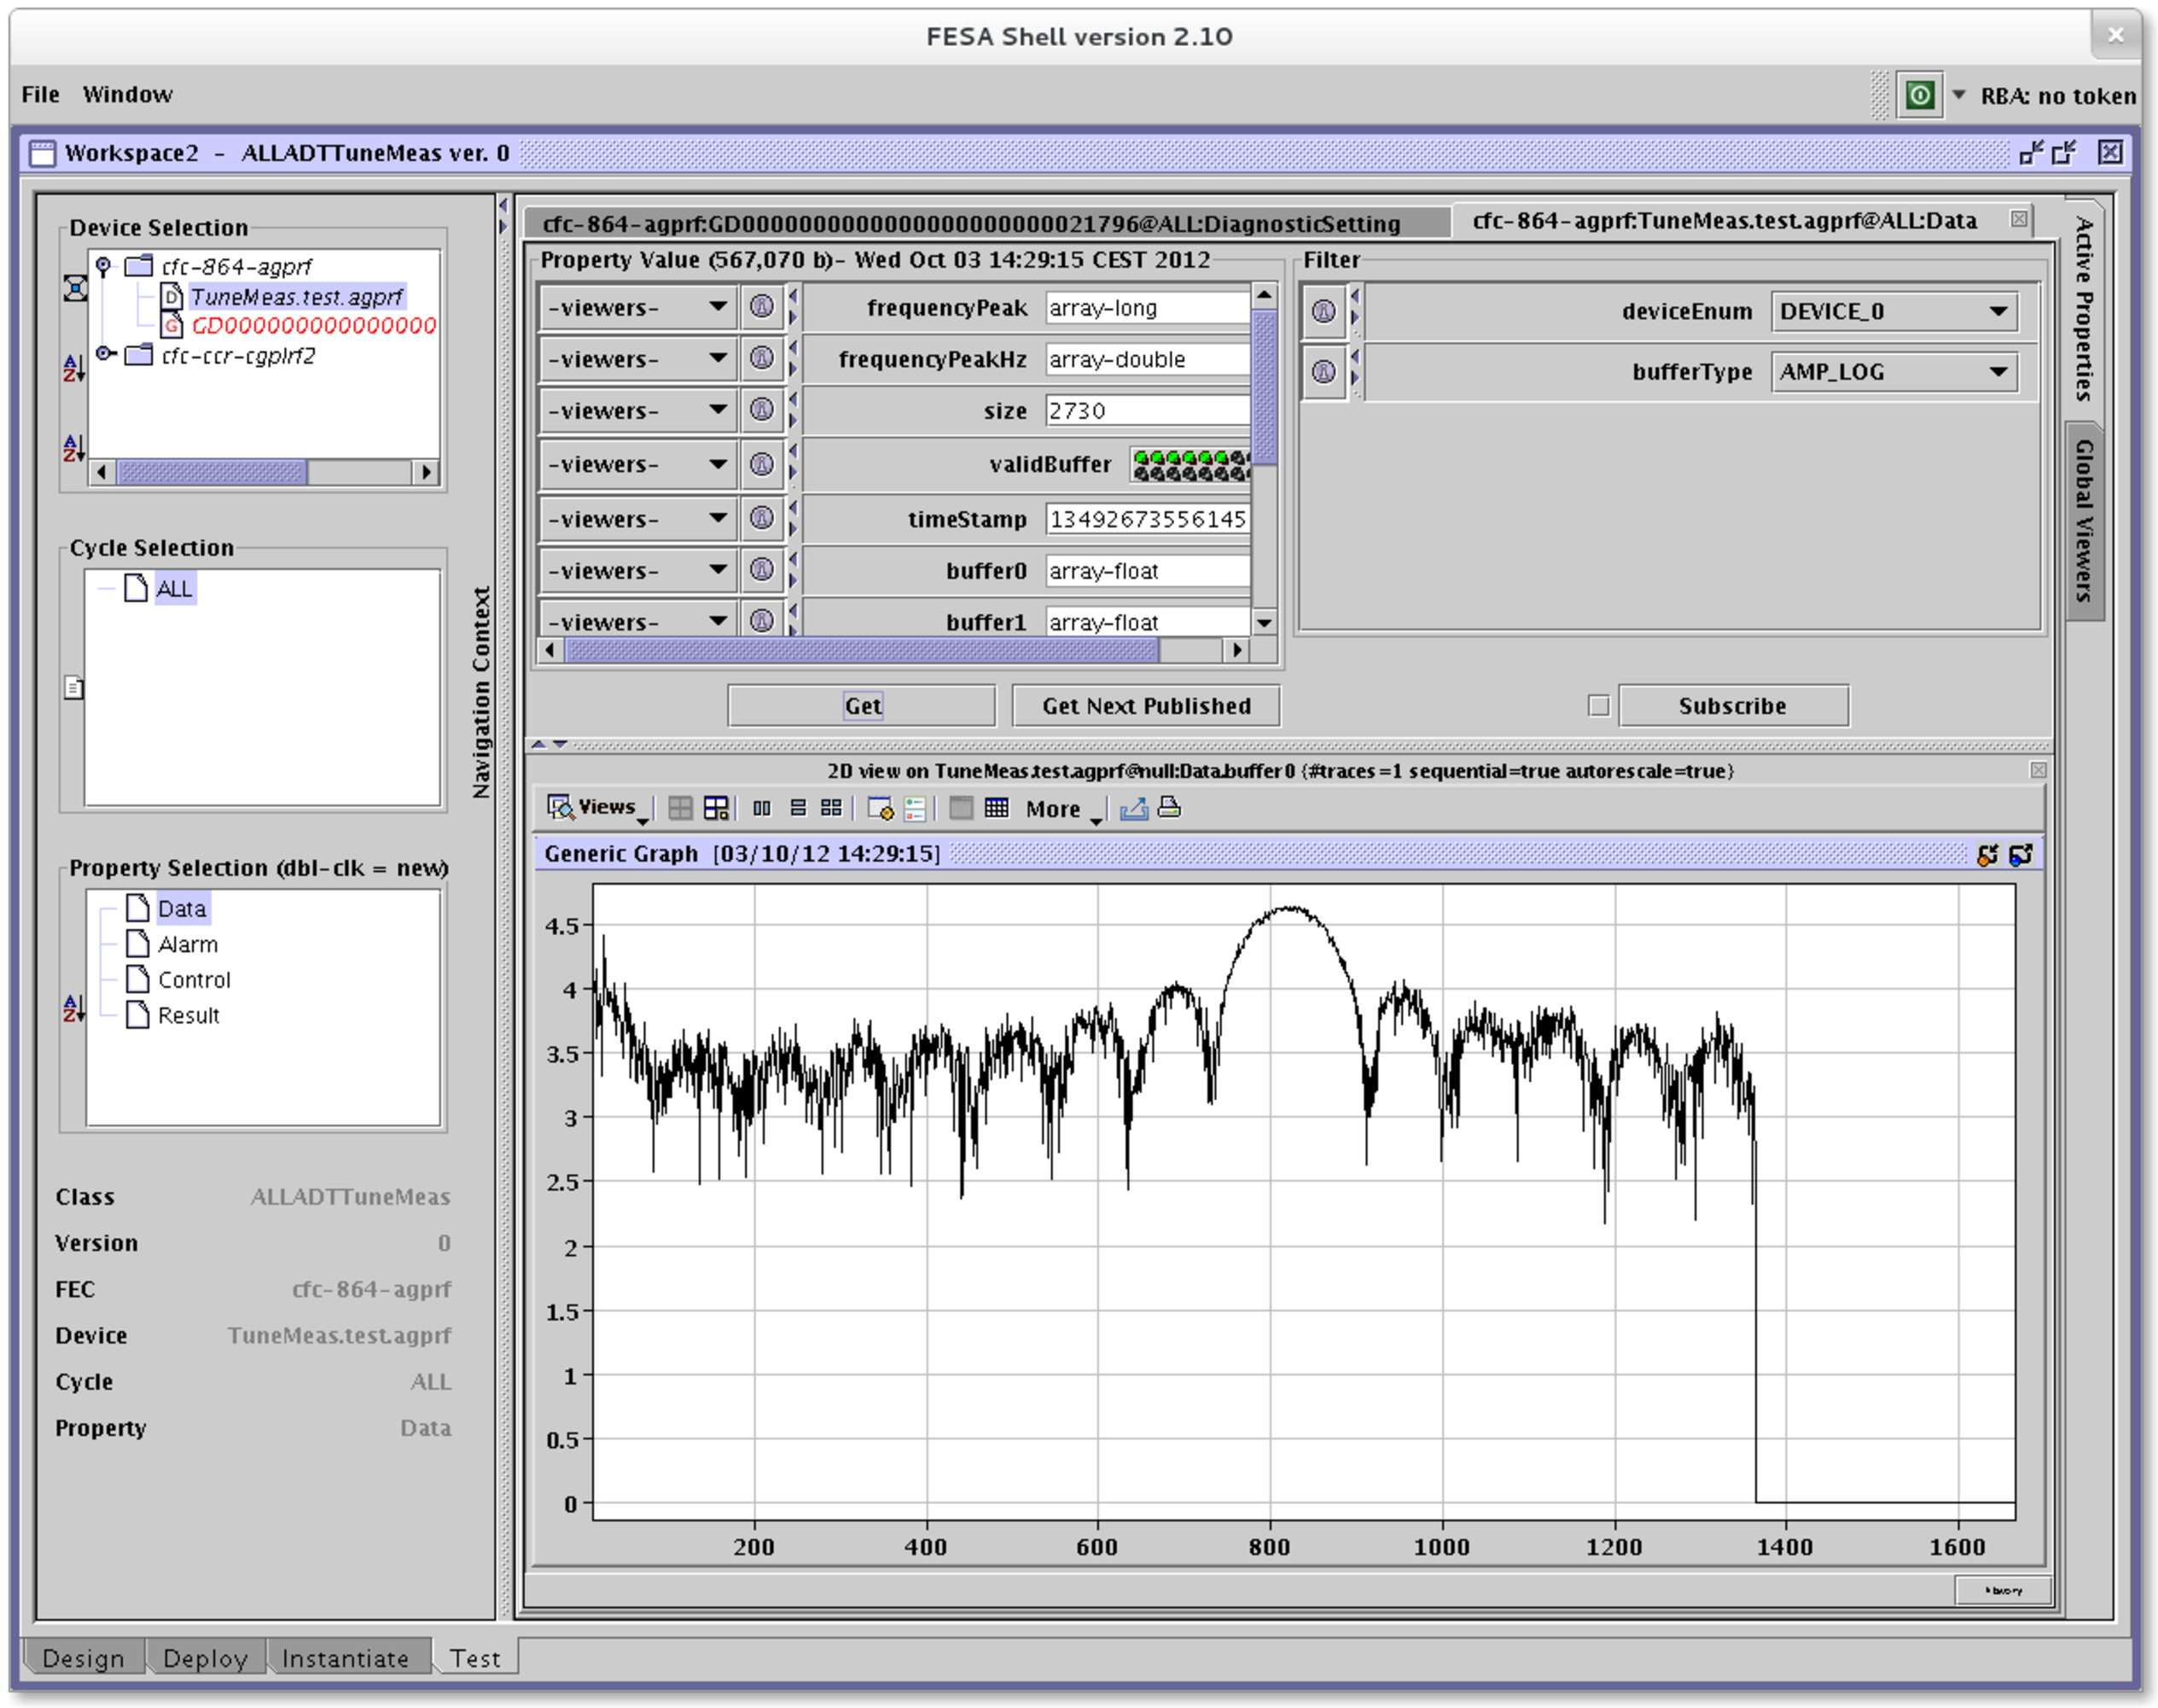
\includegraphics[scale=0.25]{amplitude_log.pdf}
	\label{fig:tuneacq}
	\end{figure}

	The acquisition software uses the \gls{CMW}, a library used at \gls{CERN} to communicate between different layers of the accelerators control software, to connect to the the ADTDPSU control software and get the data when they are published (at the time of interrupt).

	It is then able to compute the \gls{FFT} using \gls{FFTW} and display it to the operators in the \gls{CCC} from where all the eight accelerators of \gls{CERN} are controlled. On the interface one can decide which type of graph to display and also enable saving the data files to be processed by the data analysis software.

	\subsection{Data analysis software}
	\label{sec:data_analysis_software}

	The data analysis software is a set of modules that can be enabled limit or bypassed to test the usefulness of an algorithm. The modularity of the data analysis software allow us to check the time taken by each part of the algorithm and validate it against the constraints.

	\begin{figure}[H]
	\caption{Time f\/low with different implementations and with 3000 bunches of 
	2048 points each.}
	\centering
	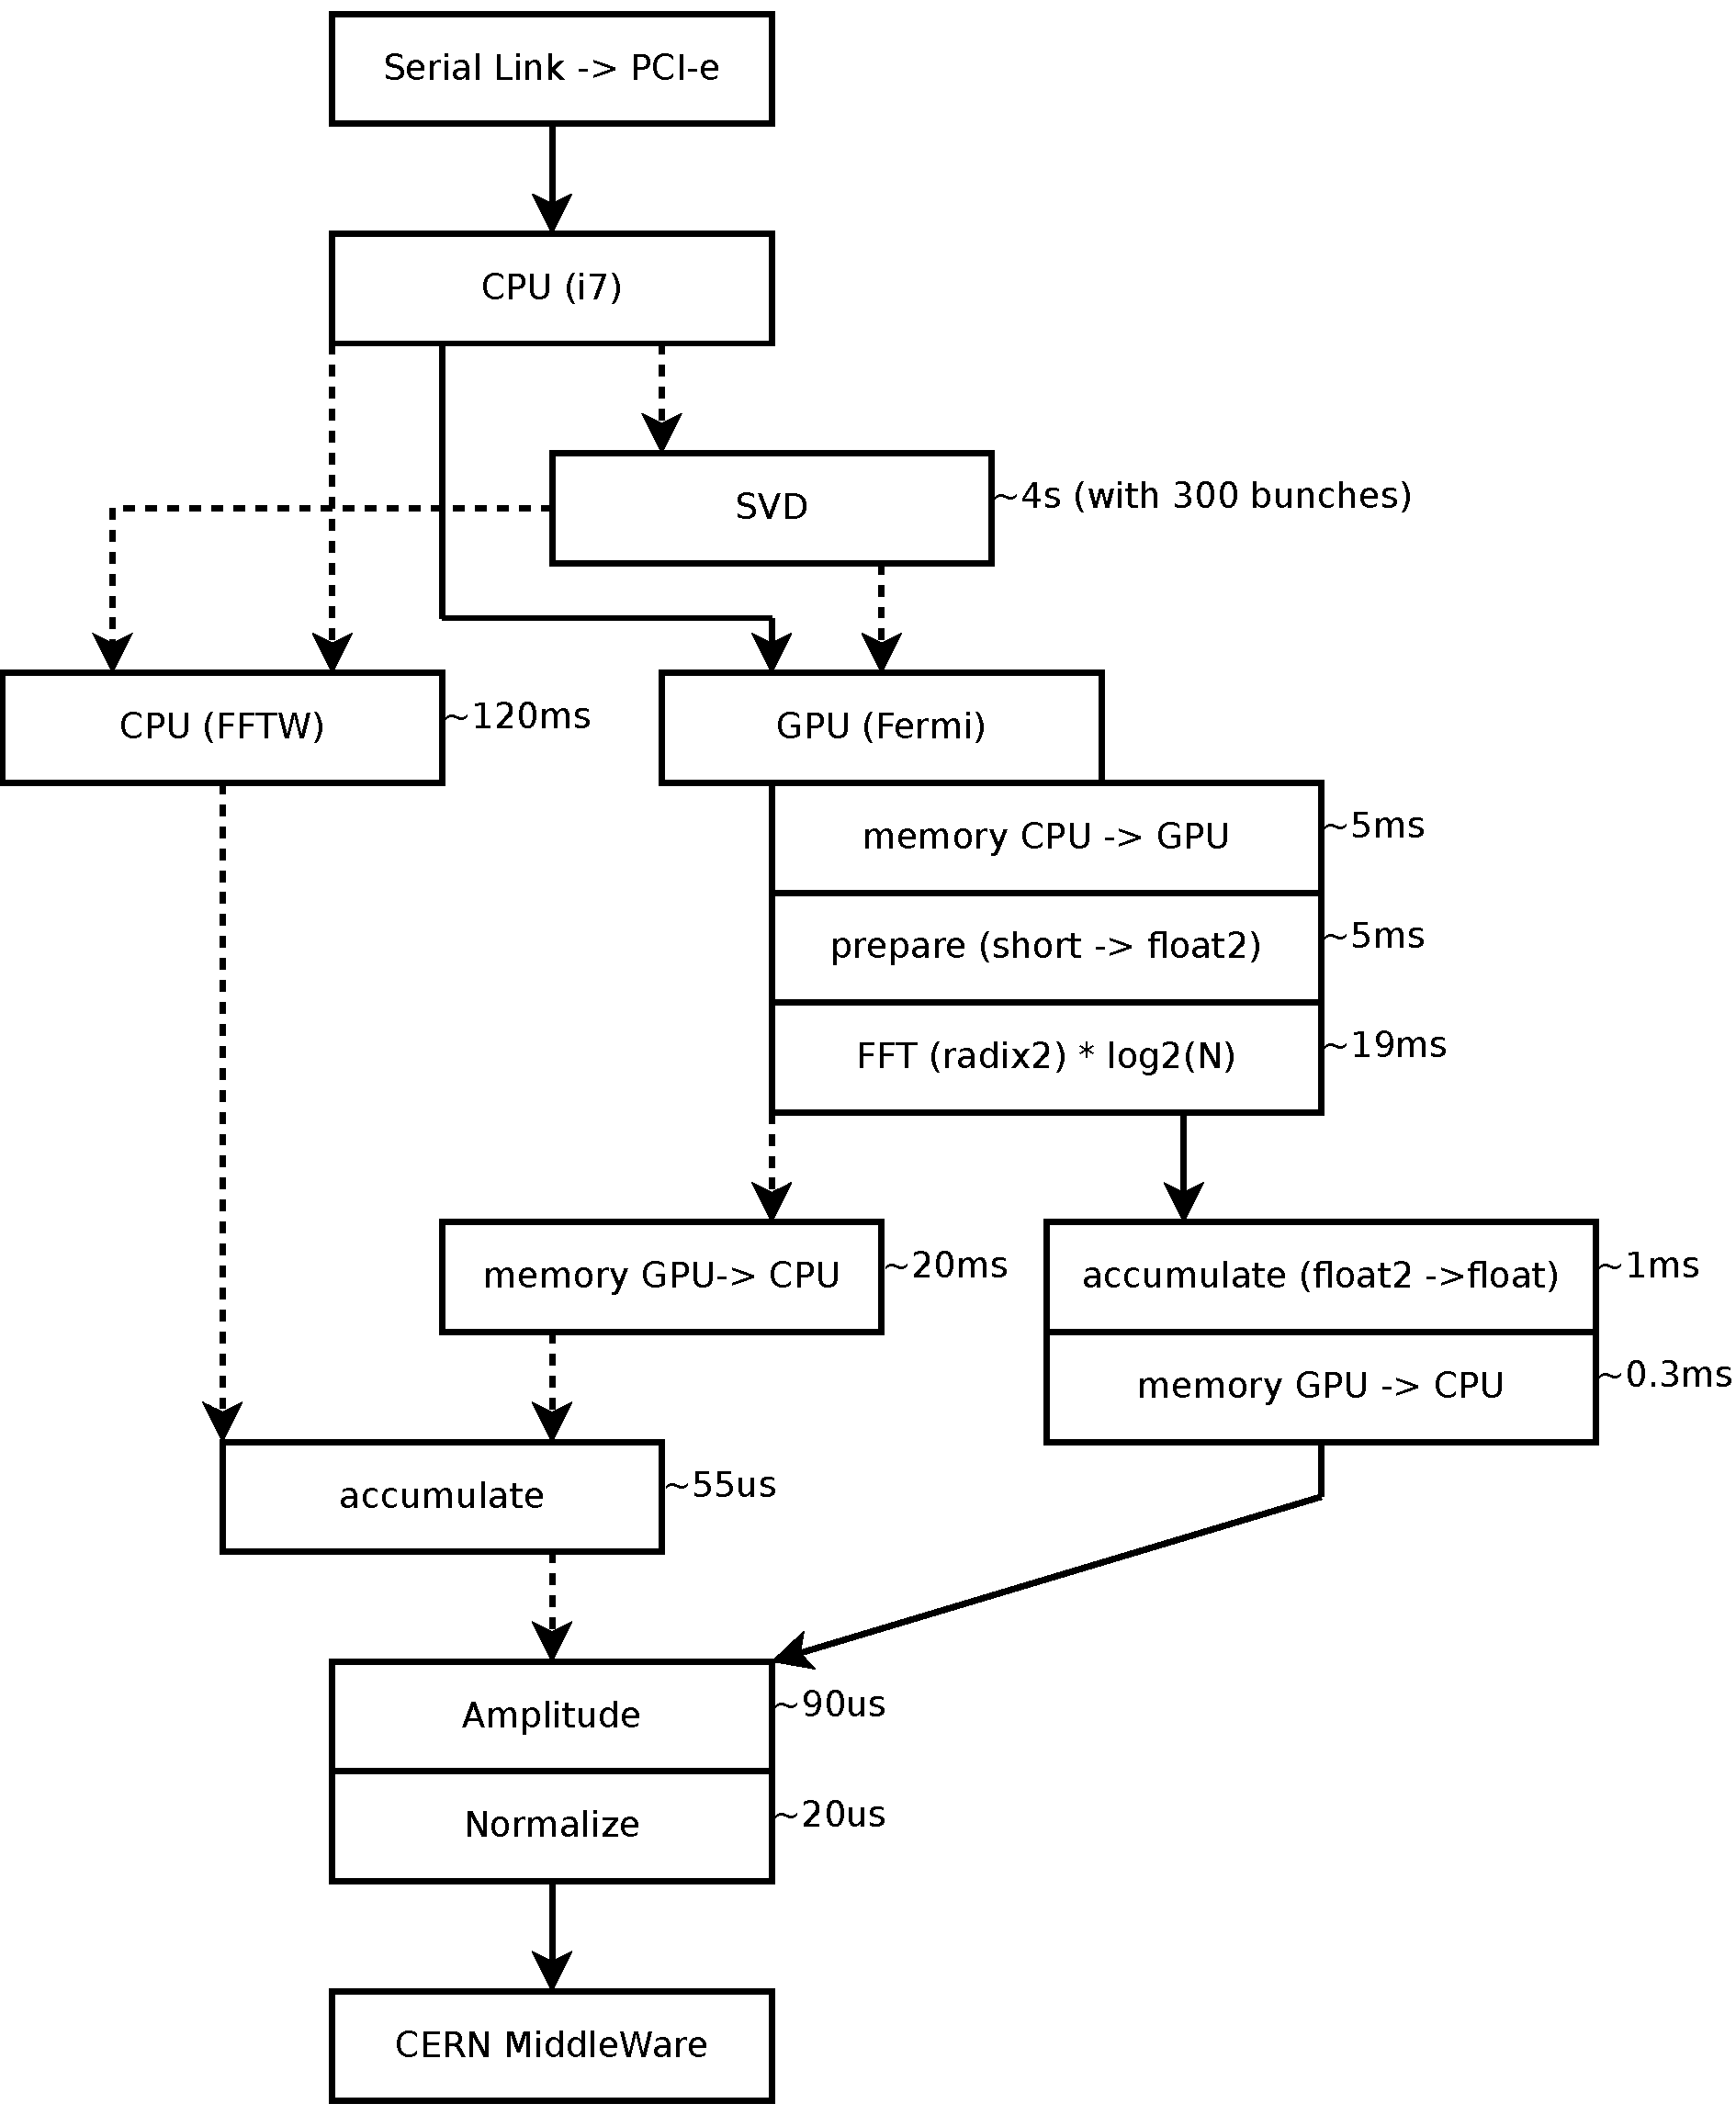
\includegraphics[scale=0.3]{PC-flow.pdf}
	\label{fig:PCFlow}
	\end{figure}

	The data is first loaded from the files that were written by the acquisition software. Then it is filtered by a notch filter as described in the notch section~\ref{sec:notch}. And finally to the different algorithms as shown in the figure~\ref{fig:PCFlow}.

	First optional step is \gls{SVD} this as described in Rama Calaga PHD thesis ``Linear Beam Dynamics and Ampere Class Superconducting RF Cavities at RHIC''\cite{calaga06} and Wolfgang H{\"o}f\/le\cite{HofleChamonix12} should reduce noise in the signal, result are shown in section~\ref{sec:SVD}.

	The \gls{FFT} are either using the \gls{GPU} or using the \gls{CPU}, actually you could use \gls{OpenCL} on the \gls{CPU} and test the whole \gls{OpenCL} path. The different path are due to memory copying, in the case of computation made on the \gls{GPU} one has to move the data from the \gls{CPU} central memory to the \gls{GPU} memory. This will described in section~\ref{sec:FFT}.

	To have a clear image and to combine the real and imaginary part of the \gls{FFT} we use the amplitude. It has been validated in the acquisition software as been the best metric, but could be changed at will in the final version. The amplitude is described in section~\ref{sec:amplitude}.

	The accumulation over all theses bunches is done, which will give an average spectrum.

	The normalization step is only present for displaying the spectrogram (see section~\ref{sec:spectrogram}) and will not be needed for the final version.
 
\section{Notch filter}
\label{sec:notch}

A notch filter is used to cut the low frequencies. It does not change anything for the high frequencies. It will not be used in the final version for reason of storing untreated data. For every sample it takes the present sample and subtract the next element. 

$$y_{[n]} = x_{[n]} - x_{[n + 1]}$$

As visible on formula one value is dropped at the end of the data set but as we are using radix 2 \glspl{FFT} the data is cut to a power of 2.

This is a differential filter and as we are only interested into the higher frequency this has no incidence on our results and allow for a better visualization of the spectrograms.

\section{FFT}
\label{sec:FFT}

The Fourier transform is a mathematical operation that moves a function from a temporal domain to a frequency domain using an integral relation. In our case we are treating sampled signals for which the integrals reduce to a summation, and the transform is referred as \gls{DFT}. The specific term ``\gls{FFT}'' refers to a fast algorithm to compute the \gls{DFT} when for example the number of samples equals $N$ a power of 2.

	\subsection{Definition}

	The \gls{DFT} is a discrete transform. It transform a series of complex numbers into another series the \gls{DFT}, of the original series.

	$$ x_0,...,x_{N -1} \in \mathbb{C} $$

	$$ X_{k} = \displaystyle\sum\limits_{n = 0}^{N -1} x_{n}e^{-i 2 \pi k \frac{n}{N}} $$

	In order to compute the \gls{DFT} one must compute $N$ number of values $N$ times. The complexity is in order of $N$ times $N$ multiplication~:

	$$ \mathcal{O}(N^{2}) $$

	The most commonly used \gls{FFT} algorithms are based on a divide-and-conquer approach similar to the algorithm of Cooley and Turkey~\cite{Cooley65}. The computation of a \gls{DFT} of length N is done by splitting the input sequence into a fixed small number of subsequences, compute their \gls{DFT}, and assemble the outputs to build the final sequence. If the split and assembly are linear in time the complexity becomes~:

	$$ \mathcal{O}(N \log_{2}(N)) $$

   	\subsection{FFTW}

   	\Gls{FFTW} is an implementation of the \gls{DFT} that adapts the algorithm to the hardware in order to maximize the performance~\cite{fftw05}. It is widely regarded as one of the fastest implementation of an \gls{FFT} on a \gls{CPU}.

   	It was selected as a reference for our the implementation, as \gls{OpenCL} can be run on directly on a \gls{CPU} is it possible to compare the time performances between the \gls{OpenCL} code running on \gls{CPU} and the \gls{FFTW} version see section~\ref{sec:perf}.

   	It is under GPL license, can be purchased from the \gls{MIT} for commercial purposes and is used in many commercial and scientific package and software. As an example it is used in the MATLAB.

   	\subsection{FFT with OpenCL on GPU}

   	The \gls{FFT} version used in the software is derived from Eric Bainville's version. This is the reference implementation of \gls{FFT} on \gls{OpenCL} and is now the version distributed by Apple\cite{bainville11}. For the sake of simplicity restrict ourself to the radix~2 version of the implementation.

   	On \gls{GPU} the \gls{OpenCL} result is the same than the one using \gls{FFTW} with the advantage to be faster on recent \gls{GPU}. The kernel is called a number of times equal to the size of the vector and then 11 times in the case of 2048 points ($\log_{2}{2^{11}} = 11$). A second dimension is used to pass the multiple vector.

   	\subsection{FFT with OpenCL on a CPU}

   	As \gls{OpenCL} is also able to run on a \gls{CPU} we used the same code than the one used on a \gls{GPU} on a \gls{CPU} yielding same results. It is interesting to note that the time is very similar to the implementation using \gls{FFTW}.

\section{Amplitude}
\label{sec:amplitude}

The amplitude is the length of the complex vector composing the \gls{FFT}; it is equal to the euclidean norm. 

$$ \mid x + i y \mid \equiv \sqrt{x^2 + y^2}$$ 

There are different ways to compute the norm of a 2-dimensional vector in \gls{OpenCL} and all of them seem to work equally well in our test.

\section{SVD}
\label{sec:SVD}

It was suggested by Rama Calaga to use \gls{SVD} in order to diminish the noise and improve the visibility of the tune in the frequency domain. The idea is to take the raw data and use the multiple bunches as a second dimension of the matrix $M$ using SVD, $M$ containing turn by turn data. One can suppress the values in the singular value matrix ($\Sigma$) that are off a certain scale, recompose the $M'$ matrix with less noise.

$$M = U \Sigma V^{T}$$ 

This was first tested in the framework of this work on generated data by Wolfgang H{\"o}f\/le~\cite{HofleEvian10}. Unfortunately we have only 6 bunches in our dataset per acquisition so it is not possible to make this work with the present set up. The $\Sigma$ matrix will only be 6 by 6 and it is not easy to suppress values with a noticeable impact on the signal to noise ratio.

Taking more than one acquisition can at least give some idea on the speed of processing and feasibility. The SVD was implemented using the GNU Scientific Library (with double precision float for the SVD). Speed efficiency is difficult to estimate as we can see on table~\ref{tab:SVD} for the same number of sample, 100 in this table, we have a big variation of speed if we try to use different acquisitions.

\begin{table}[H]
	\caption{SVD speed correlation with acquisitions bunches for a 100 by 2048 $M$ matrix}
	\label{tab:SVD}
	\centering
	\begin{tabular}{|l|l|l|}
		\hline
			Bunches & Acquisitions & Time \\
		\hline
			5 & 20 & 0.15 s \\
			4 & 25 & 0.30 s \\
			2 & 50 & 2.04 s \\
			1 & 100 & 16.9 s \\
		\hline
	\end{tabular}
\end{table}

So it is very difficult to estimate the time the computation would take with the real data. We have to keep in mind that these computation where done using double precision as single would probably be enough, these computation were also done using a single thread (SVD is quite difficult to parallelize) and only done on \gls{CPU}.

There is a way to make these computation on \gls{GPU}\cite{Lahabar09} and the estimation is that is would be around 5 times better than on a \gls{CPU}.

\section{Performances}
\label{sec:perf}

Computations were made with an accumulation to simulate the number of bunches that could be present in the final version (2880). As 6 bunches were acquired we used 500 successive acquisitions to make, close to the maximum of 2880.

Different strategies were used to try to improve the performance as shown in Figure~\ref{fig:PCFlow}. Pipelining was also used (not used on the Figure as it is difficult to estimate time when using pipelining) and tested on different type of hardware.

The hardware used was mainly the Tesla M2090 based on a Fermi chip. This chips has more cores than a CPU and we can see an improvement with respect to computing speed as shown in Table~\ref{tab:speed}. Table~\ref{tab:fermi} shows the characteristics of the Tesla Fermi card family.

\begin{table}[H]
	\caption{NVIDIA Fermi hardware available on the market}
	\floatfoot{Source : NVIDIA\cite{nvidia}}
	\label{tab:fermi}
	\centering
	\begin{tabular}{|l|l|l|}
		\hline
			Features & Tesla M2090 & Tesla M2075 \\
		\hline
		\hline
			Peak double performance & 665 Gflops  & 512 Gflops \\
		\hline
			Peak single performance & 1331 Gflops & 1030 Gflops \\
		\hline
			Memory bandwidth (ECC off) & 177 GB/sec & 150 GB/sec \\
		\hline
			Memory size (GDDR5) & 6 GB & 6 GB \\
		\hline
			CUDA cores & 512 & 448 \\
		\hline
	\end{tabular}
\end{table}

However, if we have a look on the different cards that are available today on the market we see that the new generation should provide even better result and are available today. These cards show around 5 times the number of \gls{CUDA} core and around 10 times the number of \gls{flops} as shown in Table~\ref{tab:kepler}.

\begin{table}[H]
	\centering
	\caption{NVIDIA Kepler hardware available on the market}
	\floatfoot{Source : NVIDIA\cite{nvidia}}
	\label{tab:kepler}
	\begin{tabular}{|l|l|l|l|}
		\hline
			Features & Tesla K20X & Tesla K20 & Tesla K10 \\
		\hline
		\hline
			Peak double performance & 1.31 Tflops & 1.17 Tflops & 190 Gflops \\
		\hline
			Peak single performance & 3.95 Tflops & 3.52 Tflops & 4577 Gflops \\
		\hline
			Memory bandwidth (ECC off) & 250 GB/sec & 208 GB/sec & 320 GB/sec \\
		\hline
			Memory size (GDDR5) & 6 GB & 5 GB & 8GB \\
		\hline
			CUDA cores & 2688 & 2496 & 3072 \\
		\hline
	\end{tabular}
\end{table}


   \subsection{Pipelining}

   To improve the performances one of the options is to remove all waiting time between the different operations on the \gls{GPU}, as shown in Figure~\ref{fig:PCFlow}. The different operations done on the \gls{GPU} that are done sequentially can be pipelined.

   Pipelining mean that one will not wait for all the sub-operations to be finished for a certain task on a data set, but will already start treating the next set. The first operation is copying the memory from the \gls{CPU} to the \gls{GPU} which takes a certain time. As soon as some of the data is copied the computing could start.

   In \gls{OpenCL} the different commands are queued and this command queue can be flushed (with the command endQueue). To make the pipelining work the only thing to do is to only flush at the end when all the computing has been queued. Of course some attention should be kept to avoid problems with modules writing or reading data that has not yet been read or written.

   In our case this means that the copying of the data from the \gls{CPU} to the \gls{GPU} the preparation of the data, the \gls{FFT} itself, and the amplitude computation, the accumulation and getting back the values to the \gls{CPU} are queued together in one go.

   That allows us to have a 3 to 10\% improvement on the performances, but it is difficult then to estimate the computing time of individual steps consequently the values shown in Figure~\ref{fig:PCFlow} are without pipelining.

   \subsection{Memory}

   Copying memory from and to the \gls{GPU} can be expensive time wise, as shown in Figure~\ref{fig:PCFlow}. Copying 3000 times 2048 values in short (2 bytes) takes around 10 ms. This is the reason why it is important to make the accumulation on the \gls{GPU} and avoid the \gls{FFT} computation of 3000 times 2048 complex values in float (8 bytes). It would have cost at least 40 ms to copy these values back to the \gls{CPU}. 

   The 20 ms shown in Figure~\ref{fig:PCFlow} correspond to half the values because we can cut half of the result as the \gls{FFT} computed it in real only so the result is mirrored.
	
   \subsection{Time}

	\begin{table}[H]
		\caption{Speed for 3000 acquisitions of 2048 points}
		\centering
		\label{tab:speed}
		\begin{tabular}{|l|lrrcr|}
			\hline
				Device & Type & Threads & Speed [GHz] & Pipeline & Time [ms] \\
			\hline
			\hline
				Xeon X5650 & FFTW & 12 & 2.67 & N/A & 291 \\
				Xeon X5650 & OpenCL & 12 & 2.67 & enable & 284 \\
				Xeon X5650 & OpenCL & 12 & 2.67 & disable & 288 \\
			\hline
				i7-3720QM & FFTW & 8 & 2.6 & N/A & 310 \\
				i7-3720QM & OpenCL & 8 & 2.6 & enable & 272 \\
				i7-3720QM & OpenCL & 8 & 2.6 & disable & 273 \\
			\hline
			\hline
				Tesla M2090 & OpenCL & 512 & 1.3 & enable & 35 \\
				Tesla M2090 & OpenCL & 512 & 1.3 & disable & 37 \\
			\hline
				GeForce 650M & OpenCL & 384 & 0.9 & enable & 355 \\
				GeForce 650M & OpenCL & 384 & 0.9 & disable & 365 \\
			\hline
		\end{tabular}
	\end{table}

	Time performances were computed using the timing library from boost \cite{boost} on different hardware, \glspl{GPU} and \glspl{CPU}, with and without pipeline enable as shown on table \ref{tab:speed}.

	The time performances between \gls{FFTW} and \gls{OpenCL} on a \gls{CPU} are very close, hence the radix 2 implementation used must be good and we can hope the performances on \gls{GPU} could then be fairly compared with \gls{FFTW}.

	On a dedicated \gls{GPU} like the Tesla M2090  the performances are around 10 times better than on a modern \gls{CPU}. This is very encouraging and means that on the latest generation hardware we should be able to achieve even better performances.
	
\section{Spectrogram}
\label{sec:spectrogram}

A Spectrogram is a time-varying spectral representation of a signal. the signal is transformed via \gls{FFT} from time domain to spectral domain, each transformation makes a line in this case and is tagged with the time of the acquisition. the amplitude is used to have a single representation of both real and imaginary part of the result.

As we do a normalization by acquisition at the end of the computing we have a representation of the highest value with highest color (white) and if the amplitude is respectively weaker we have a darker representation of the color (black). To have a finer grain in representation intermediate color was chosen in this case blue as you can see in figure \ref{fig:squeeze} \ref{fig:ramp} and \ref{fig:adt_off}.

\begin{figure}[H]
	\caption{Spectrogram with ADT off on the 16 October 2012 on vertical beam 1 during squeeze and collision}
	\label{fig:squeeze}
	\centering
	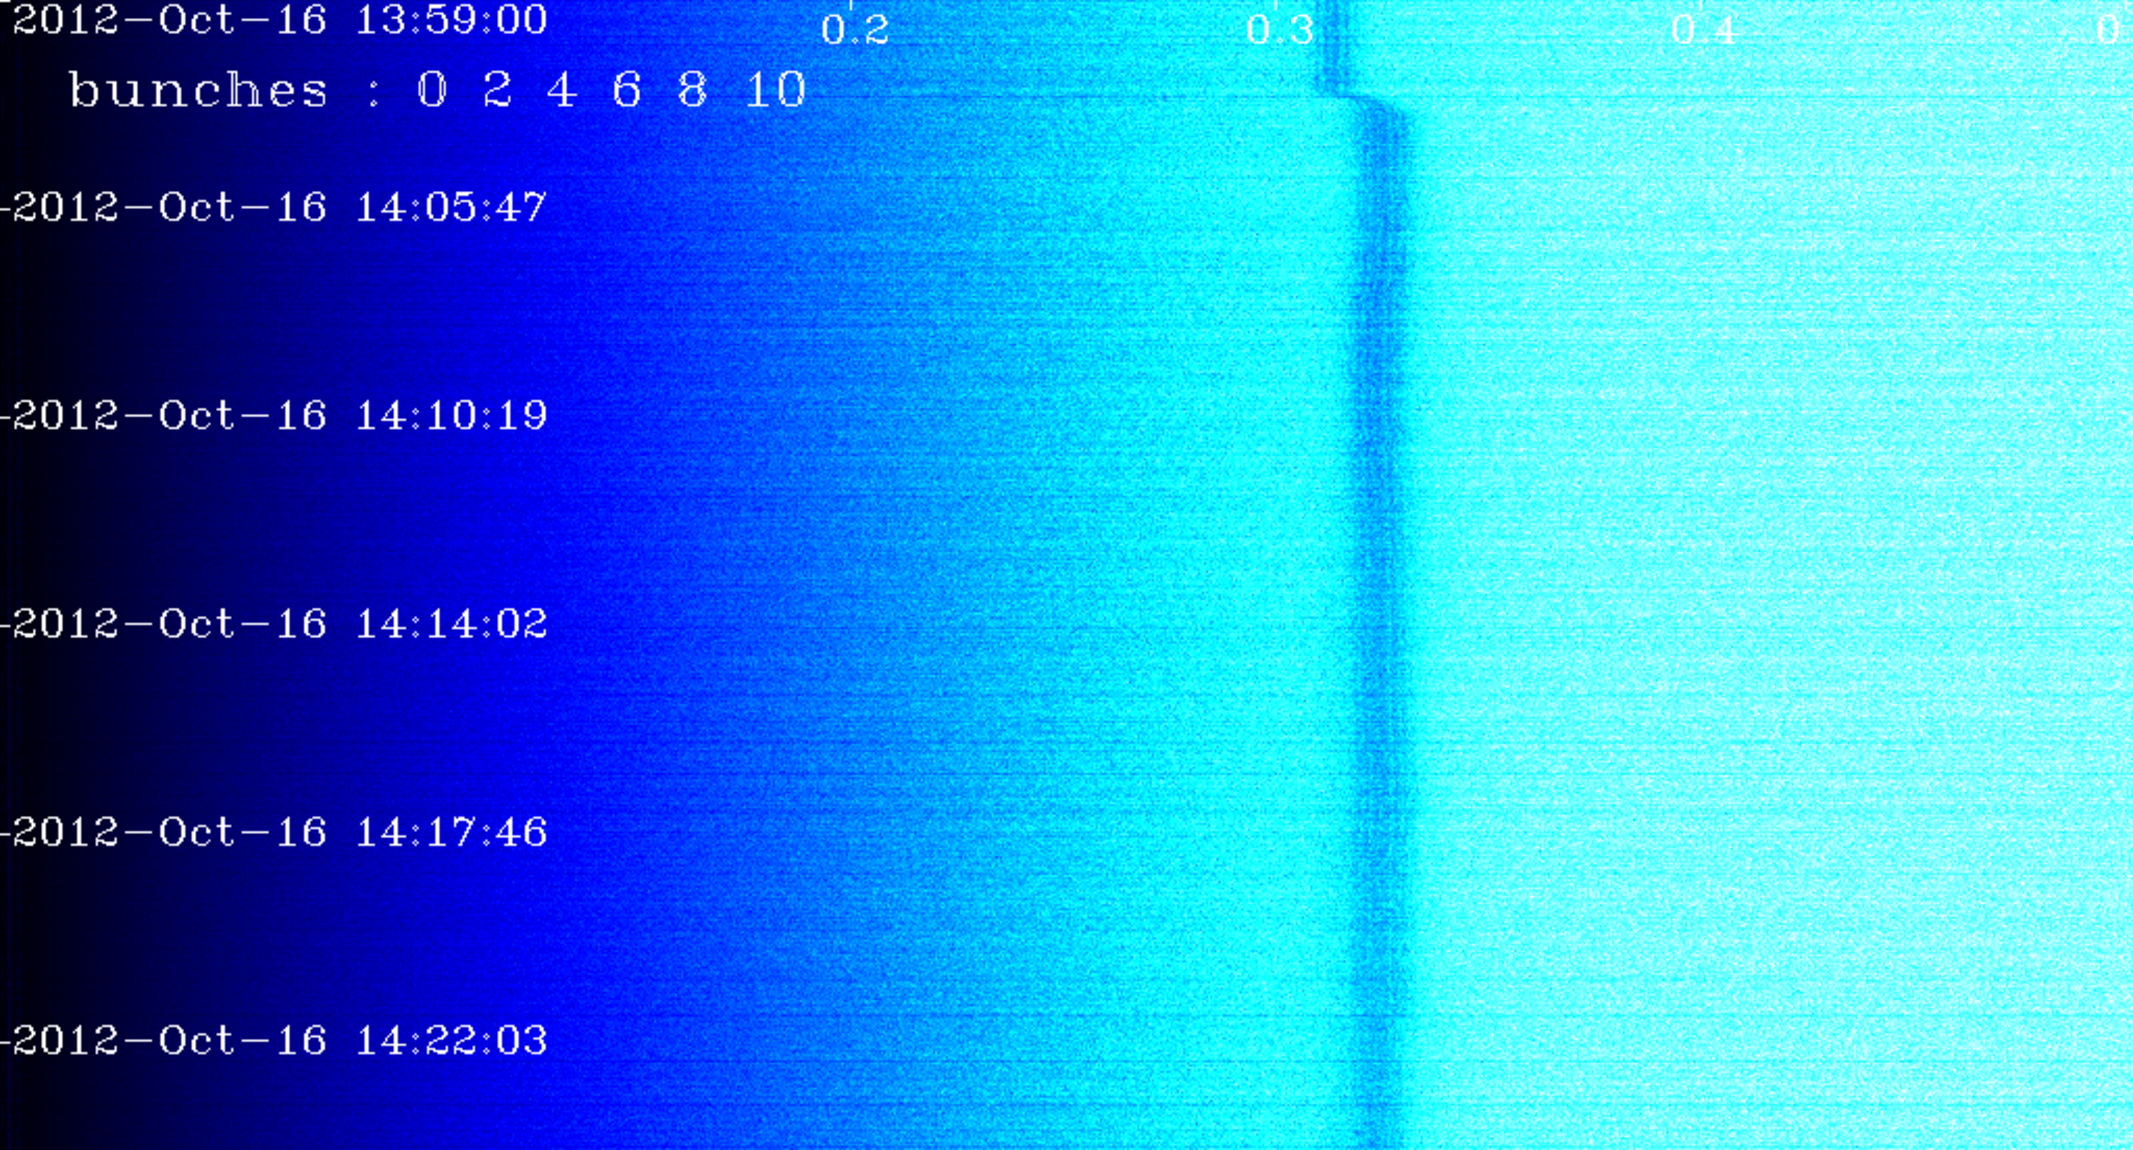
\includegraphics[scale=0.3]{md-121016-vb1-m1-6bunches-10acc-1359-1425-collision.pdf}
\end{figure}

The Spectrogram allow us to clearly see a mark in the signal that correspond to a region where the tune is suppose to be.